% Created 2018-08-06 Mon 14:16
% Intended LaTeX compiler: pdflatex
\documentclass[a4paper]{article}
\usepackage[utf8]{inputenc}
\usepackage[T1]{fontenc}
\usepackage{graphicx}
\usepackage{grffile}
\usepackage{longtable}
\usepackage{wrapfig}
\usepackage{rotating}
\usepackage[normalem]{ulem}
\usepackage{amsmath}
\usepackage{textcomp}
\usepackage{amssymb}
\usepackage{capt-of}
\usepackage{hyperref}
\usepackage{minted}
\usepackage[margin=0.8in]{geometry}
\usepackage{amssymb,amsmath}
\usepackage{fancyhdr} %For headers and footers
\pagestyle{fancy} %For headers and footers
\usepackage{lastpage} %For getting page x of y
\usepackage{float} %Allows the figures to be positioned and formatted nicely
\restylefloat{figure} %and this command
\usepackage{hyperref}
\hypersetup{urlcolor=blue}
\usepackage{titlesec}
\setcounter{secnumdepth}{4}
\usepackage{minted}
\setminted{frame=single,framesep=10pt}
\chead{}
\rhead{\today}
\cfoot{}
\rfoot{\thepage\ of \pageref{LastPage}}
\usepackage[parfill]{parskip}
\usepackage{subfig}
\hypersetup{colorlinks=true,linkcolor=black, citecolor=black}
\usepackage{framed}
\author{NH, CN, HO, JD}
\date{\today}
\title{Domestication Draft}
\hypersetup{
 pdfauthor={NH, CN, HO, JD},
 pdftitle={Domestication Draft},
 pdfkeywords={},
 pdfsubject={},
 pdfcreator={Emacs 27.0.50 (Org mode 9.1.9)},
 pdflang={English}}
\begin{document}

\maketitle


\section{Introduction}
\label{sec:org700d30b}
<Not sure on>




\clearpage
\section{Results}
\label{sec:org3d5bf2d}

\begin{figure}[htbp]
\centering
\includegraphics[width=8cm]{/home/nathan/Dropbox/NPPC/Domestication/Figures/fig1.png}
\caption{\label{fig:org4a7a3b6}
Wheats}
\end{figure}

\subsection{Domestication}
\label{sec:org6165991}
Previous studies have shown that domestication has led to an increase in grain size (\cite{Gegas2010,Peng2011}), though the precise changes were not identified.
Here we have shown that both emmer and einkorn species have both increased significantly in grain width and depth, with length remaining similar
(our analysis has shown a 36\% in einkorn and 49\% probability in emmer that the mean values of grain length overlap over domestication state).

\subsection{Ploidy}
\label{sec:orgd2c20ca}

\subsubsection{Domestication/Wild}
\label{sec:orgcc75f0c}

\begin{figure}[htbp]
\centering
\includegraphics[width=16cm]{/home/nathan/Dropbox/NPPC/Domestication/Figures/fig2.png}
\caption{\label{fig:org683801b}
Einkorn Traits}
\end{figure}

\begin{figure}[htbp]
\centering
\includegraphics[width=16cm]{/home/nathan/Dropbox/NPPC/Domestication/Figures/fig4.png}
\caption{\label{fig:orge2c4b6a}
Emmer Traits}
\end{figure}

Across ploidy in domesticated einkorn and emmer, 2N and 4N respectively, grain parameters are generally significantly different. The one parameter which
we report almost no significant change in is grain width. A \(p=0.17\) in difference in sample mean width was calculated using the Welch T-test. A probability of mean overlap of 50\%
was observed for width at an individual level.

\textbf{Citations needed to verify?}


In wild species of einkorn and emmer no significant change is seen in individual grain length or width;
Across population means non-significance is observed in grain length and width (all of which have \(likelihood > 33\%\) of overlapping means and \(p>0.01\)).

Significant changes are seen in depth, volume and surface area of grains (\(p<0.01\)), indicating that the change in depth effected overall grain shape.

\textbf{Citations needed to verify?}

\begin{figure}[htbp]
\centering
\includegraphics[width=8cm]{/home/nathan/Dropbox/NPPC/Domestication/Figures/fig3.png}
\caption{\label{fig:orgba8a8b4}
Einkorn PCA}
\end{figure}

\begin{figure}[htbp]
\centering
\includegraphics[width=8cm]{/home/nathan/Dropbox/NPPC/Domestication/Figures/fig5.png}
\caption{\label{fig:org77d5d95}
Emmer PCA}
\end{figure}


\section{Methods}
\label{sec:org2468c2a}
\subsection{Materials}
\label{sec:org495e4d9}
< Plants which were used > \ldots{}
\subsubsection{How they were sourced}
\label{sec:orgfbbe8e8}
\subsubsection{Any additional information}
\label{sec:org2f52b19}

\subsection{3D Scanning of Spikes}
\label{sec:org3c0aa2e}

From the genotypes selected, fully dried,
representative spikes were chosen for micro-CT scanning.
Spikes were placed in plastic holders (34x70mm tubes) and imaged using a a μCT100 scanner (Scanco Medical, Switzerland).

The imaging system was configured with an X-ray source ranging from 20 to 100 kVp,
a detector of 3072 x 400 elements. A resolution of 68.8 micro-meters per pixel was used for all scans.


\subsection{Computational Methods}
\label{sec:org36dc96c}

Using software developed for previous wheat studies by the National Plant Phenomics Centre (\cite{Hughes2017}) . New and novel additions are implemented in the watershedding and segmentation processes, of the existing pipeline, in order to work with the more complex primitive species of wheat.

Due to the optimised resolution of the imaging technique (68.6\textmu{} meters per pixel) objects can appear connected which are not, particularly in primitive grain. A three dimensional watershedding algorithm is used to correct any objects which appear connected when they should not be.

The software, developed in MATLAB (\cite{MATHWORKS2017}), is freely available at <insert link to NPPC>.

\paragraph{Pipeline}
\label{sec:org3d92b5e}
The scanning and MATLAB routine pipeline:

\begin{figure}[htbp]
\centering
\includegraphics[width=12cm]{/home/nathan/Dropbox/NPPC/Domestication/Figures/Suppl/matlab.png}
\caption{\label{fig:orgb4dd527}
Pipeline}
\end{figure}

\subsubsection{Morphometric Features}
\label{sec:orga16b3bd}

The features/phenotypes used are extracted during the imaging process.

\begin{itemize}
\item Length is calculated using the major axis of the whole grain.
\item Width and depth are the major and minor axis of a cross section, found by selecting the grain's midpoint.
\item Volume is a complete connected pixel count per grain
\item Surface area is a single pixel perimeter calculation mapped in 3 dimensions
\item Length X Depth X Width is a post-image-processing value calculated by the interaction between the three dimension descriptors.
\end{itemize}

Values used in statistical functions and measurements are presented as metric units, derived from \textmu{}-CT image pixel values. The equation:\ref{eq:org5f9c827} is presented here.
\begin{align}
\label{eq:org5f9c827}
  &\begin{aligned}
mm = \frac{pixel \times 68.8}{1000}
  \end{aligned}
\end{align}

\subsubsection{Error Removal}
\label{sec:org0d50ab6}
The data were checked for false positives, this is done by first removing outliers which are found by the 0.025 upper and lower percentiles of the data. Additionally constraints are applied to the data based on findings from previous studies \cite{Hughes2017}, this adds robustness.

\subsubsection{LWD}
\label{sec:orga500c80}
An additional phenotype is created to describe the interaction between the geometric parameters; the interaction is described in equation:\ref{eq:orgc5f306d}.

 \begin{align}
\label{eq:orgc5f306d}
   &\begin{aligned}
\text{geometry interaction} = length \times depth \times width
   \end{aligned}
 \end{align}

\subsubsection{Image Analysis Methods}
\label{sec:org84dfb69}
\textbf{\emph{I could provide a lot of info on this, but weary of going off-track, more can be added (or taken away) if needed, what's in comp methods could be enough I think.}}

\subsection{Bayesian Modelling}
\label{sec:orgabcb0fd}
To provide deeper insight into the size of change or similarity in hypothesis testing, a Bayesian model is used. To estimate probability of two samples containing the same mean the method uses Bayes theorem (\(P(A|B) \propto P(B|A) \times P(A)\)) \cite{Kruschke2012} along with Markov-Chain-Monte-Carlo (MCMC) to draw random samples from a normal population.

From Krusches' method a percentage likelihood of difference is produced.

\subsection{Linear Modelling}
\label{sec:orgf1d6972}

A linear model allowed for an R\(^{\text{2}}\) value of 0.91 in einkorn species when predicting domestication status.

\subsubsection{Draft Supplemental figure for dom}
\label{sec:org31bd52c}

\begin{figure}[htbp]
\centering
\includegraphics[width=18cm]{/home/nathan/Dropbox/NPPC/Domestication/Figures/Suppl/Reg_Dom.png}
\caption{\label{fig:orge81711e}
is showing a multiple regression of r=.91 by using length, width and depth to correctly ID domestication status.}
\end{figure}


\subsubsection{Draft Supplemental figure for volume}
\label{sec:orgaa95095}
\begin{figure}[htbp]
\centering
\includegraphics[width=12cm]{/home/nathan/Dropbox/NPPC/Domestication/Figures/Suppl/Regression_Analysis_Vol.png}
\caption{\label{fig:org68e6e98}
Showing the importance of 3rd dimension of depth}
\end{figure}

\subsubsection{Least Squares Model}
\label{sec:orgdf053ac}

Equation, where the intercept (\(\beta_{\text{0}}\)) has been set by surface area

$$ Y = \beta_0 + \times \beta_1 length \times \beta_2 depth \times \beta_3 width  + \epsilon $$

\subsubsection{Misc}
\label{sec:org2e15438}
The model produced an r\(^{\text{2}}\) value by:

$$1- \frac{\sum\limits_{i=0}^{n}{r^2}}{\sum\limits_{i=0}^{n}{(y_i - \overline{y})^2 }}$$



\section{Misc Information to fold into discussion?}
\label{sec:orgff21b2d}

Fuller has evidenced that grain volume is used when initially identifying wheat grain which is recovered as being domesticated \cite{Fuller2007} .
Therefore justification for our model is very useful.

On the other hand \cite{Willcox2004} found that barley is much harder to identify from it's domesticated relatives.
 Volume is not significantly different! Which fits perfectly with our results!

Wondering outloud, with the wild 2n/4n an oberserved change in surface area. Would there be a
reason for why grains would want to develop a larger surface area? Alternatively we can work off-of volume, as that changes also

\clearpage
\section{Data Tables}
\label{sec:org3ba29ac}

\subsection{einkorn}
\label{sec:org936d935}
\begin{figure}[htbp]
\centering
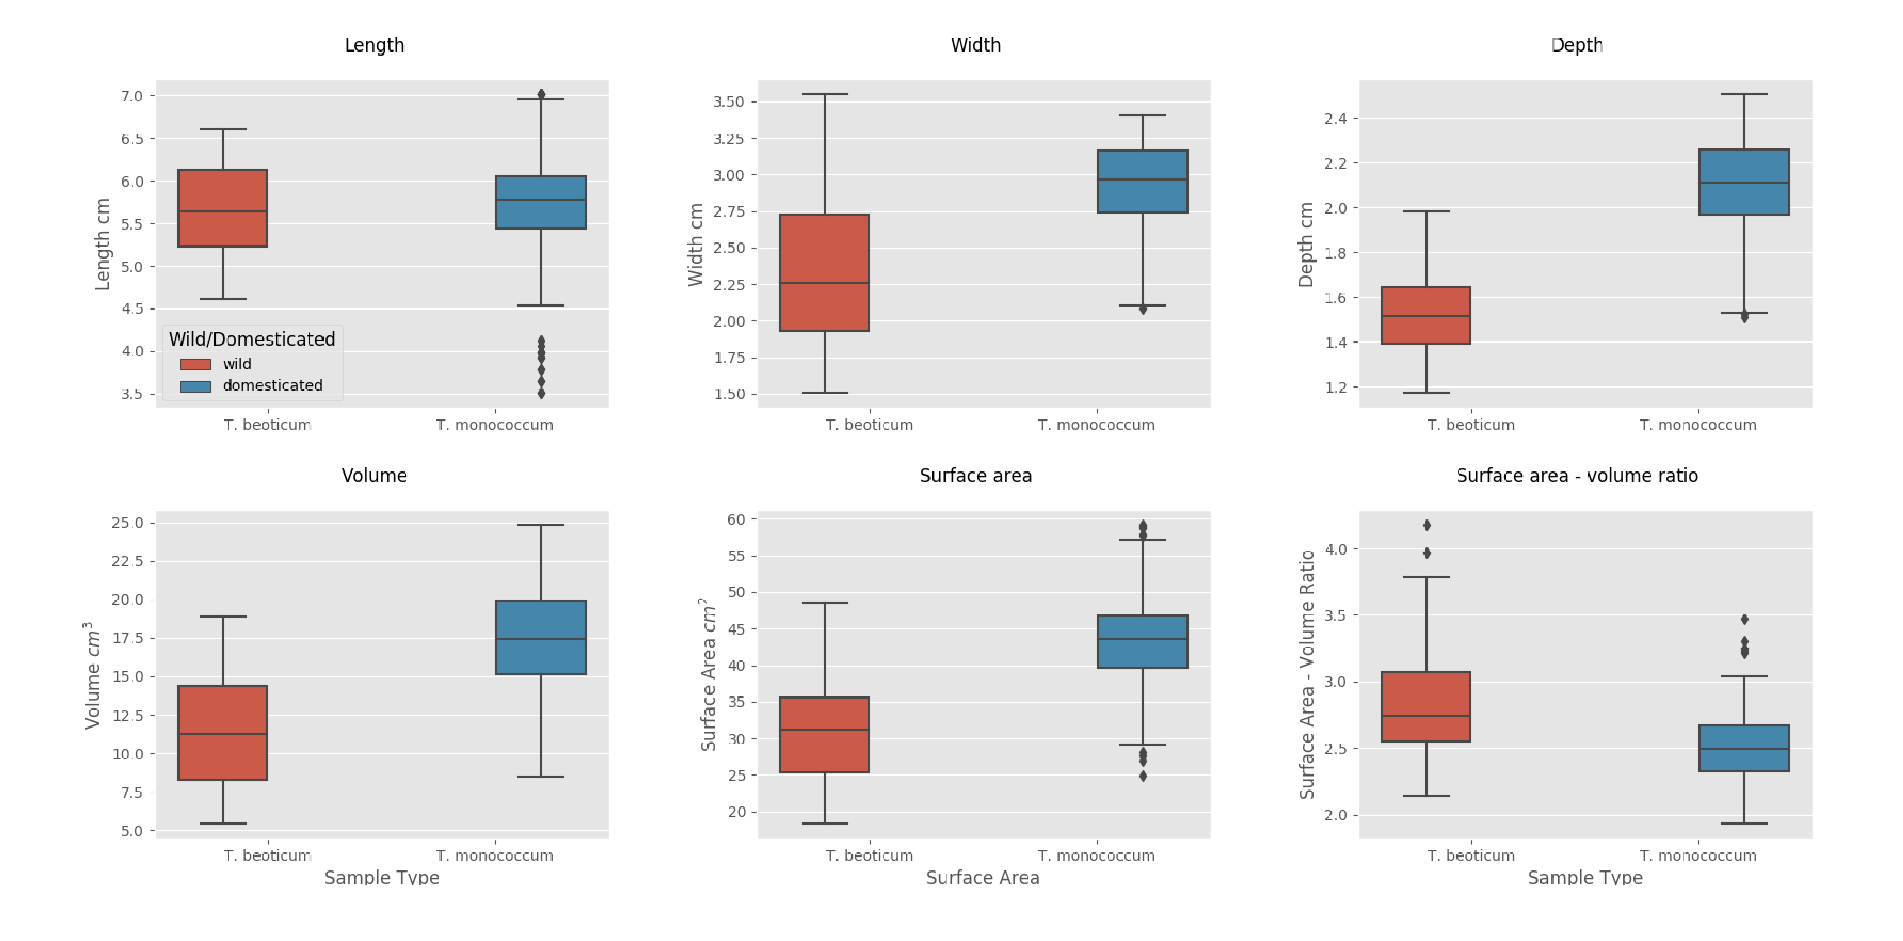
\includegraphics[width=.9\linewidth]{./einkorn.png}
\caption{\label{fig:org066959b}
einkorn table}
\end{figure}


\subsection{emmer}
\label{sec:org2630b92}
\begin{figure}[htbp]
\centering
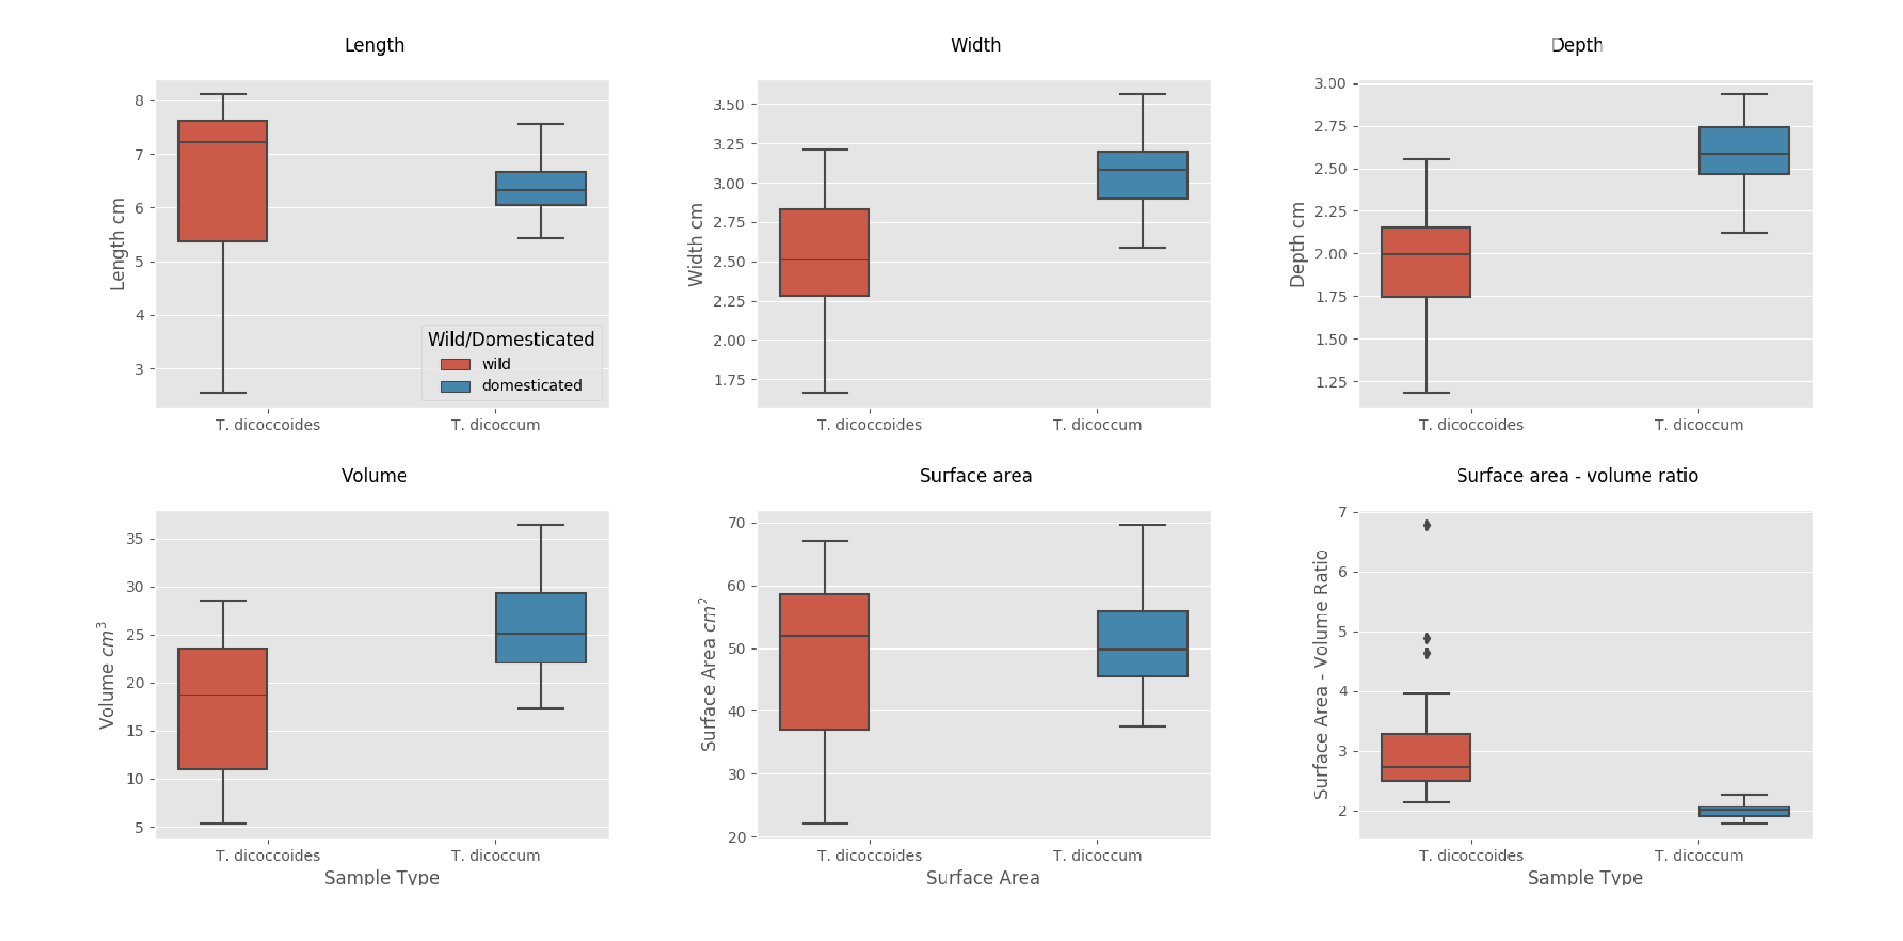
\includegraphics[width=.9\linewidth]{./emmer.png}
\caption{\label{fig:org810fb56}
emmer table}
\end{figure}

\clearpage


\subsection{Barley}
\label{sec:org5b46b88}
\begin{figure}[htbp]
\centering
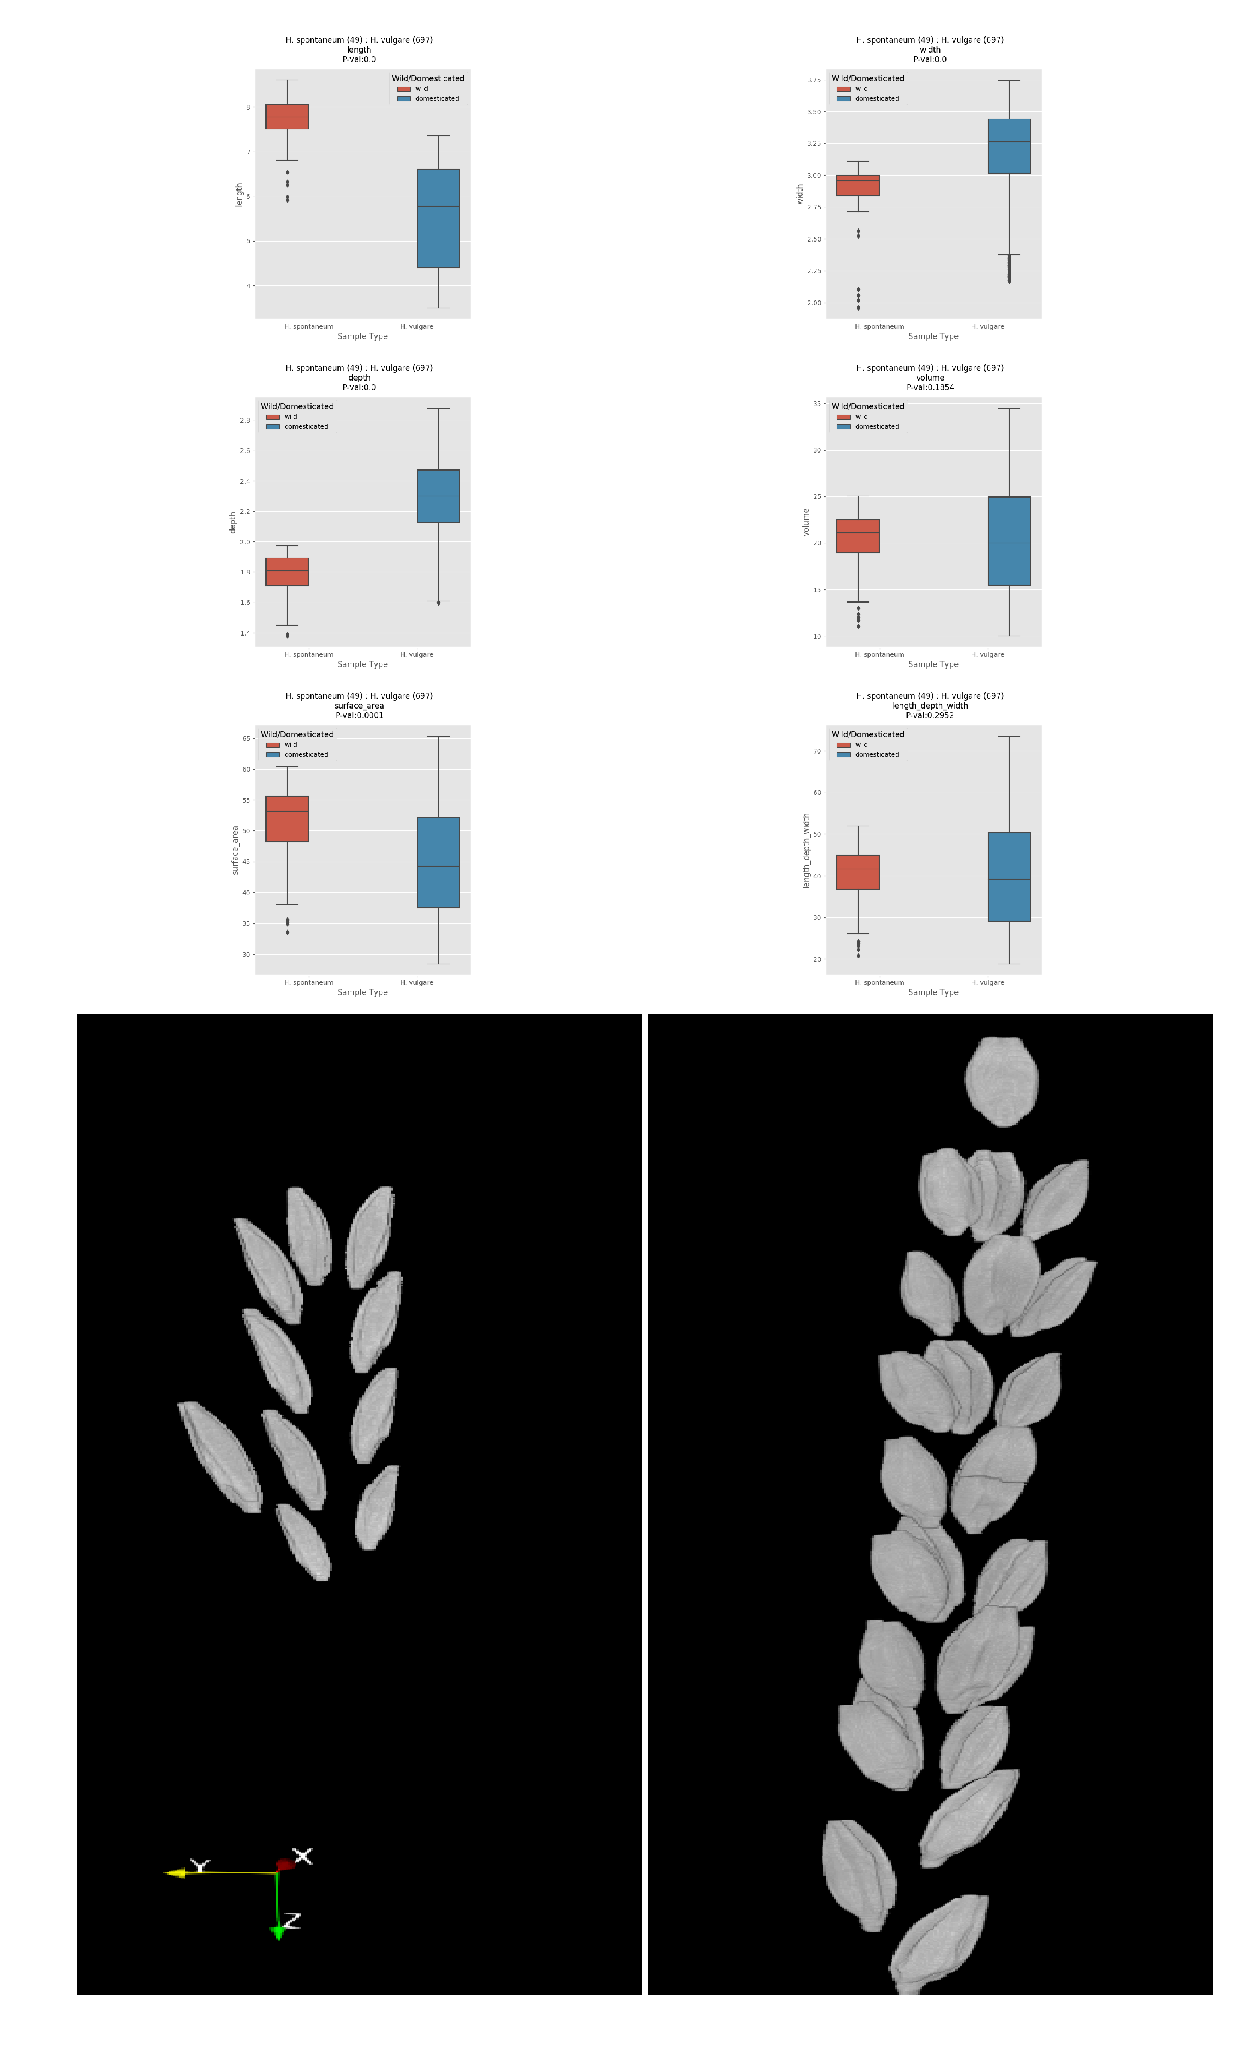
\includegraphics[width=.9\linewidth]{./barley.png}
\caption{\label{fig:orgfeee5a0}
barley table}
\end{figure}


\subsection{Domesticated 2N, 4N}
\label{sec:org93af86d}
\begin{figure}[htbp]
\centering
\includegraphics[width=.9\linewidth]{./dom.png}
\caption{\label{fig:org0dbb402}
domesticated 2N, 4N table}
\end{figure}

\clearpage
\subsection{Wild 2N, 4N}
\label{sec:org9992cc0}
\begin{figure}[htbp]
\centering
\includegraphics[width=.9\linewidth]{./wild.png}
\caption{\label{fig:org7255b0d}
wild 2N, 4N  table}
\end{figure}

\clearpage
\bibliography{library}
\bibliographystyle{unsrt}
\end{document}